\section{Zielsetzung}
\label{sec:Zielsetzung}
Es werden die Brennweiten verschiedener Sammellinsen und eines
Linsensystems bestimmt.

\section{Theorie}
\label{sec:Theorie}
Da Linsen meist aus einem dichteren Material als ihre Umgebung bestehen,
werden Lichtstrahlen beim Ein- und Austreten aus der Linse gebrochen.
Unterschieden wird in der Optik zwischen Sammel- und Zerstreuungslinsen.
Sammellinsen sind konvex geformt und bündeln parallele Strahlen im
Brennpunkt $f$. Da Bildweite $b$ und Brennweite $f$ positiv sind,
entsteht ein reelles Bild hinter der Sammellinse, wie in Abbildung 1
zu erkennen ist.
\begin{figure}[H]
\label{eq:sammellinse}
\center
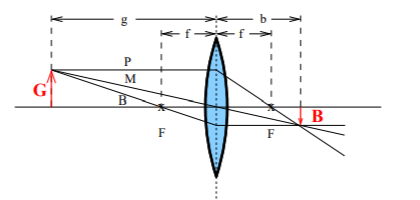
\includegraphics[scale=0.75]{sammellinse.png}
\caption{Bildkonstruktion an einer Sammellinse. \cite[S.1]{kent}}
\end{figure}

\noindent Zerstreuungslinsen sind konkav geformt und erzeugen wegen ihrer negativen
Brennweite $f$ ein virtuelles Bild vor der Linse.  Dies ist in Abbildung 2
dargestellt.

\begin{figure}[H]
\label{fig:zerstreuung}
\center
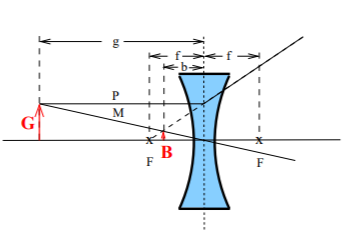
\includegraphics[scale=0.75]{zerstreuung.png}
\caption{Bildkonstruktion an einer Zerstreuungslinse.\cite[S.1]{kent}}
\end{figure}

\noindent Bisher betrachtet wurden dünnen Linsen, bei welchen sich die Konstruktion
des Bildes auf die Mittelebene der Linse reduzieren lässt. Bei dicken
Linsen, wie in Abbildung 3 zu sehen, werden zur Bildkonstruktion zwei
Hauptebenen $H$ und $H'$ eingeführt.

\begin{figure}[H]
\label{fig:dicke}
\center
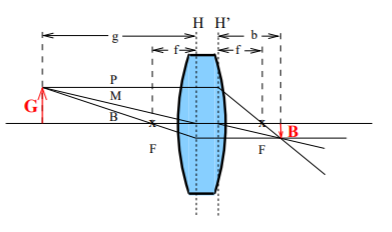
\includegraphics[scale=0.75]{dick.png}
\caption{Bildkonstruktion durch Einführung zweier Hauptebenen an einer dicken Linse.\cite[S.1]{kent}}
\end{figure}

\noindent In allen drei Fällen werden zur Konstruktion drei Strahlen verwendet. Der
Parallelstrahl $P$  läuft parallel zur optischen Achse vom Gegenstand zur
Mittel- bzw Hauptebene, wird gebrochen und wird dann zum Brennpunktstrahl.
Der Brennpunktstrahl $B$ verläuft durch den Brennpunkt bevor er an in der
Linse gebrochen wird und dann zum Parallelstrahl wird. Der Mittelpunktstrahl
$M$ verläuft vom Gegenstand durch die Mitte der Linse und ändert dabei
seine Richtung nicht.
\noindent Für Bildgröße $B$, Gegenstandsgröße $G$, Bildweite $B$, Gegenstandsweite
$g$ und Abbildungsmaßstab $V$ gilt das Abbildungsgesetz:
\begin{equation}
\label{eqn:abbildungsgesetz}
V = \frac{B}{G} = \frac{b}{g}.
\end{equation}
Aus diesem wiederum folgt für dünne Linsen die Linsengleichung:
\begin{equation}
\label{eqn:linsengleichung}
\frac{1}{f} = \frac{1}{b} + \frac{1}{g},
\end{equation}
wobei $f$ die Brennweite der Linse darstellt.
Wenn Brennweite, Gegenstandsweite sowie Bildweite zur jeweiligen Hauptebene bestimmt werden, behält die Linsengleichung auch für dicke
Linsen ihre Gültigkeit.
\noindent Experimentell lässt sich die Brennweite $f$ außerdem durch die Methoden
von Bessel und Abbe bestimmen.
Bei der Methoden nach Bessel wird der Abstand zwischen Bild und Gegenstand
konstant gehalten und es werden die beiden Linsenpositionen bestimmt, bei
denen das Bild scharf ist. Bei dieser symmetrischen Linsenstellung sind
Bild- und Gegenstandsweite vertauscht, es gilt also $b_1 = g_2$ und
$b_2 = g_1$. Mit Hilfe des Abstands $e = g_1 + b_1 = g_2 + b_2$ zwischen
Bild und Gegenstand und dem Abstand $d = g_1 - b_1 = g_2 -b_2$ zwischen
den beiden Linsenpositionen ergibt sich für die Brennweite $f$:
\begin{equation}
\label{eq:bessel}
f = \frac{e^2 - d^2}{4e}.
\end{equation}

\noindent Bei der Methode nach Abbe wird die Brennweite eines Linsensystems aus
Sammel- und Zerstreuungslinse bestimmt. Dazu wird die Lage der Hauptebenen
benötigt. Diese lässt sich über den Abbildungsmaßstab $V$ bestimmen. Dazu
werden Bild- und Gegenstandsweite zu einem beliebigen Referenzpunkt $A$
gemessen, wie in Abb. 4 dargestellt. Die Lage der Hauptebenen $h$ und
$h'$, sowie die Brennweite $f$ ergeben sich dann aus:
\begin{equation}
\label{eq:abbe1}
g' = g+h = f\left(1+ \frac{1}{V}\right) + h
\end{equation}
\begin{equation}
\label{eq:abbe2}
b' = b+h' = f \left(1+ V \right)+h'.
\end{equation}

\begin{figure}[H]
\label{fig:abbe}
\center
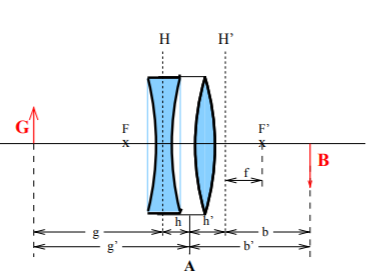
\includegraphics[scale=1]{abbe.png}
\caption{Methode nach Abbe zur Bestimmung der Brennweite. \cite[S.5]{kent}}
\end{figure}

\noindent Die vereinfachende Annahme der ausschließlichen Brechung an der Mittel-
bzw. Hauptebene gilt nur für achsennahe Strahlen. Durch achsenferne
Strahlen, welche stärker gebrochen werden, können Abbildungsfehler
auftreten, durch die das Bild unscharf wird. Diese sphärische Abberration lässt sich
beispielsweise durch eine Blende, welche die achsenfernen Strahlen
ausblendet, beheben.
Chromatische Abberation kommt dadurch zustande, dass Licht
unterschiedlicher Wellenlänge unterschiedlich stark gebrochen wird.
